\section{Dataset creation}

The first step of any classification project, especially if it uses machine learning, is to acquire and refine data. At the time the project was proposed, it was already clear that no existing dataset would be available. This proved to be true as discussed in section \ref{sota}, where we saw that existing research focuses on WiFi and Zigbee technologies.

% -------------------------------------------------------------------------------------------------------------
\subsection{Radio setup}

This section's goal is to describe the material used to capture the communications between NFC readers and tags. The final setup is illustrated in figure \ref{fig:radio-setup}.

\begin{figure}[htp!]
  \centering
  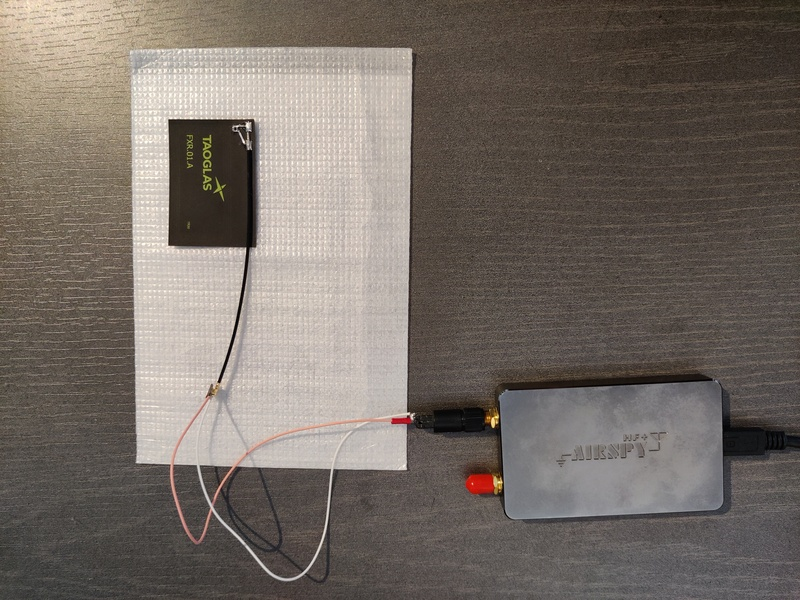
\includegraphics[scale=0.35]{figures/data_sdr-setup2.jpg}
  \caption{Airspy HF+ and antenna setup}
  \label{fig:radio-setup}
\end{figure}

\subsubsection{The SDR}

The first part of the analysis phase was conducted using a LimeSDR Mini\footnote{\url{https://www.crowdsupply.com/lime-micro/limesdr-mini}}. We used it to learn about SDR in general and to make our first recordings. In that regard it was very useful, but our model had a set of shortcomings we weren't able to accommodate. First, it became very hot very quickly, which couldn't have been good for the stability of the recording. Also, while it worked all the time for higher frequencies, it seemed to only pick up our HF signals one out of six times or so. This proved quite frustrating and attempts at tweaking the parameters in LimeSuite GUI (the device's official configuration software) generally resulted in errors.

Despite these setbacks, we were able to record communications well enough to decode the reader's transmissions, as described in section \ref{validation}. The tag's response, though, was drowned in the noise most of the time, as far as we can tell. These are the reasons why we replaced the LimeSDR Mini with the Airspy HF+\footnote{\url{https://airspy.com/airspy-hf-plus}} you can see in figure \ref{fig:radio-setup}, courtesy of Mr Joël Conus.

The Airspy HF+, as its name suggests, is built for HF (the frequency range in which NFC operates). As such, it proved a lot more stable at 13.56MHz (picking up our signal every time) and a lot less prone to heating. Most importantly, the noise level is much lower with this device, which allows us to clearly distinguish a tag's response. The only drawback is its sampling rate which can only be set at one of five values, the highest of which is 768kS/s. \cite{rtlsdr_our_2017, marks_airspy}

\begin{table}[h!]
  \centering
  \begin{tabular}{|l|l|l|l|}
    \hline
    \textbf{Name}         & \textbf{Frequency range}                                                       & \textbf{Bandwidth}                                           & \textbf{Transmitter?} \\ \hline
    \textbf{LimeSDR Mini} & 10MHz - 3.5GHz                                                                 & Up to 30.72 MHz                                                                  & Yes                        \\ \hline
    \textbf{Airspy HF+}   & \begin{tabular}[c]{@{}l@{}}HF: 9kHz - 31MHz\\ VHF: 60MHZ - 260MHZ\end{tabular} & \begin{tabular}[c]{@{}l@{}}768kHz, 384kHz, 192kHz,\\ 96kHz or 48kHz\end{tabular} & No                         \\ \hline
  \end{tabular}
  \caption{Theoretical characteristics of mentionned SDRs}
  \label{tab:pcd-inventory}
\end{table}

\subsubsection{The antenna}

As described in section \ref{nfc}, NFC uses inductive coupling rather than the more common far-field electromagnetic radiations. Because of this, our system needs a near-field antenna, which in this case is really just an inductor. A simple loop of copper wire qualifies as such, but in order for our system to be perfectly tuned to 13.56MHz, we used an industrial antenna: the Taoglas FXR.01.A\footnote{\url{https://www.taoglas.com/product/fxr01-nfc-flex-reader-antenna}}.

The antenna should be placed at least 15mm away from metallic objects, for they interfere with the magnetic field used for the communication.

As can be seen in figure \ref{fig:radio-setup}, the adapter between the SDR and the antenna is homemade using spare connectors and copper wires. The risk of interferences because of this rather unsophisticated adapter is noted, but doesn't seem to be significant later in the work.

% -------------------------------------------------------------------------------------------------------------
\newpage
\subsection{Inventory of devices}

Here, we list the devices used to create the dataset. These include the PCDs (readers) and the PICCs (tags) whose communications were captured.

In terms of readers, table \ref{tab:pcd-inventory} lists the few devices used, for documentation purposes. Of course, only one reader will be used to elaborate the final dataset, but it was useful to compare the results during the analysis phase. We weren't able to find a specific NFC chip in either smartphone's characteristics. The final dataset will be created with the help of \texttt{reader1}, as it is more recent.

\begin{table}[h!]
  \centering
  \begin{tabular}{|l|l|l|}
    \hline
    \textbf{Name}    & \textbf{Type} & \textbf{Model} \\ \hline
    \textbf{reader1} & Smartphone    & OnePlus 8      \\ \hline
    \textbf{reader2} & Smartphone    & Nokia 7+       \\ \hline
  \end{tabular}
  \caption{Inventory of PCD devices}
  \label{tab:pcd-inventory}
\end{table}

On the other hand, the list of tags and their technical details can be found in table \ref{tab:picc-inventory}. A picture of tags 1 to 7 is also provided in figure \ref{fig:tags}. As the table shows, tags 1 to 5 use the exact same chip model. Tags 1 to 8 are all NFC type A compliant, while tag 9 uses the FeliCa standard from Sony. It will be interesting to contrast the classification performance between tags of the same type and between tags of different types.

\begin{table}[h!]
  \centering
  \begin{tabular}{|l|l|l|l|l|l|l|}
    \hline
    \textbf{Name} & \textbf{NFC type} & \textbf{Standard} & \textbf{Chip}     & \textbf{Writable} & \textbf{ATQA} & \textbf{SAK} \\ \hline
    \textbf{tag1} & NFC-A             & ISO 14443-3A      & NTAG213           & Yes               & 0x0044        & 0x00         \\ \hline
    \textbf{tag2} & NFC-A             & ISO 14443-3A      & NTAG213           & Yes               & 0x0044        & 0x00         \\ \hline
    \textbf{tag3} & NFC-A             & ISO 14443-3A      & NTAG213           & Yes               & 0x0044        & 0x00         \\ \hline
    \textbf{tag4} & NFC-A             & ISO 14443-3A      & NTAG213           & Yes               & 0x0044        & 0x00         \\ \hline
    \textbf{tag5} & NFC-A             & ISO 14443-3A      & NTAG213           & Yes               & 0x0044        & 0x00         \\ \hline \hline
    \textbf{tag6} & NFC-A             & ISO 14443-3A      & Mifare Classic 1k & Yes               & 0x0004        & 0x08         \\ \hline
    \textbf{tag7} & NFC-A             & ISO 14443-3A      & Mifare Classic 1k & Yes               & 0x0004        & 0x08         \\ \hline
    \textbf{tag8} & NFC-A             & ISO 14443-4       & Mifare Classic 4k & No                & 0x0002        & 0x38         \\ \hline
    \textbf{tag9} & FeliCa            & JIS 6319-4        & RC-S967           & No                & -             & -            \\ \hline
  \end{tabular}
  \caption{Inventory of PICC devices}
  \label{tab:picc-inventory}
\end{table}

On the PICCs that are marked writable, the content is harmonized to ensure the algorithm won't use the content as a feature to identify devices.

\begin{figure}[htp!]
  \centering
  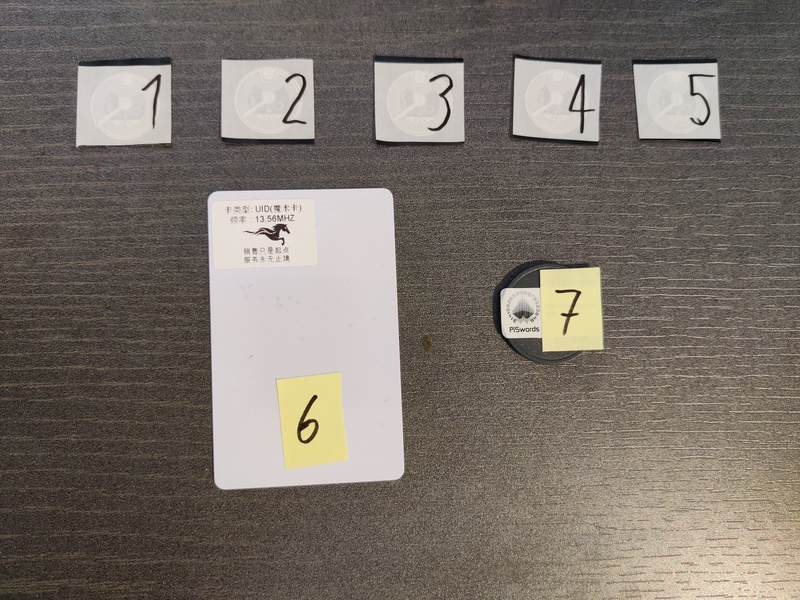
\includegraphics[scale=0.35]{figures/data_standard-tags2.jpg}
  \caption{NFC tags 1-7}
  \label{fig:tags}
\end{figure}

\subsubsection{Software used}

We used GNU Radio Companion (GRC)\footnote{\url{https://wiki.gnuradio.org/index.php/Main_Page}} for all of our experiments. It is a very versatile tool, allowing us to define software pipelines using a block interface to create flow graphs. As it compiles to python, the idea is to use it as a base for acquisition and processing scripts.

The format used by GRC's file writer is simple. It writes raw bytes into a file, alternating between the real part and the imaginary part of the sample. Both parts are written as 32 bits floating-point numbers.

On the reader (an Android smartphone), we use the NFC Tools\footnote{\url{https://www.wakdev.com/en/apps/nfc-tools.html}} app to get information about the tags and manipulate their content.

% -------------------------------------------------------------------------------------------------------------
\subsection{Dataset description}

\subsubsection{Requirements}

In order for the dataset to be robust, it needs to answer some basic criteria. The following list assumes the dataset will be used to train a machine learning model to discriminate between passive tags.

\begin{itemize}
  \item It should contain recordings of both very similar and very different devices.
  \item The data transmitted should not be a discriminating factor.
  \item The number of devices should be high enough to analyse scalability and generalization.
  \item Only one reader should be used to initiate a communication.
  \item Only one SDR should be used to capture the data.
  \item The capture's parameters should be constant across captures.
\end{itemize}

If some of those items are not met, the model trained using this data could use the content of the tags or the capture's parameters to categorize the data. It may also be unable to generalize when unknown tags appear.

\newpage
\subsubsection{Visualization of the signal}

A typical NFC communication, captured using the hardware described above, is represented in figure \ref{fig:nfc-full}. We can observe that before the reader is brought to the tag, the line is almost flat at zero. This shows a very low noise level. Then, there is a sudden surge of amplitude in the signal as the reader generates the magnetic field required for the communication. This part, referred to as the "transient portion" of the signal by \textcite{xu_device_2015} (although they talk about WiFi), might be very characteristic of the device. Then, the amplitude decreases and regular request/responses start.

\begin{figure}[htp!]
  \centering
  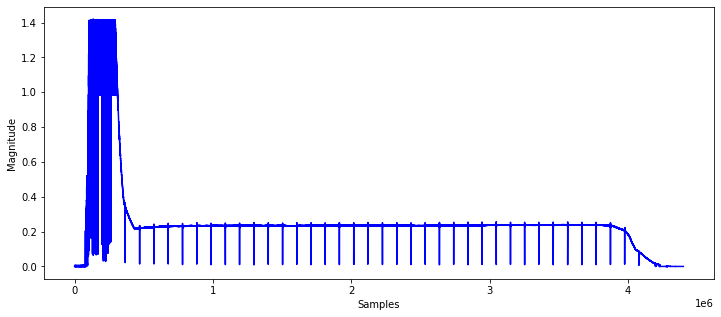
\includegraphics[scale=0.5]{figures/data_whole-transmission.png}
  \caption{NFC communication represented as magnitudes}
  \label{fig:nfc-full}
\end{figure}

In figure \ref{fig:nfc-single}, we take a closer look at one of the request/responses of the previous figure. We can clearly see a first transmission followed by a pause and then a second transmission, with smaller amplitude. This is how NFC communications work, with a request sent by the reader device followed by the tag's response through modulation of the reader's magnetic field.

\begin{figure}[htp!]
  \centering
  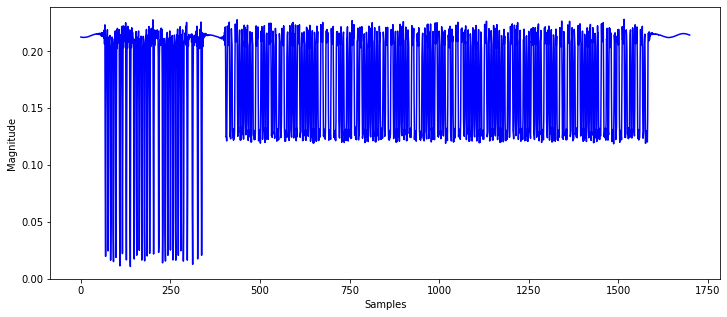
\includegraphics[scale=0.5]{figures/data_single-request-response.png}
  \caption{NFC single request/response represented as magnitudes}
  \label{fig:nfc-single}
\end{figure}

% -------------------------------------------------------------------------------------------------------------
\subsection{Validating the dataset} \label{validation}

The next step in the elaboration of the dataset is to be absolutely sure that the data is fully captured by our setup. The previous section seems to show this is the case, but to be sure we would need to decode the signal.

To do so, we need to know the modulation and coding used by the protocol. In the case of our NFC-A tags, the reader's transmissions are coded with a modified Miller code, while the tag's responses are coded with Manchester coding. Both modulate the data with On-Off Keying (OOK), which represents zeroes as no change of amplitude and ones as changes in amplitude over a given time period. \cite{wiki_off_2020}

Miller coding, as applied in NFC communications, works by mapping four symbols in the signal to a bit. A one is always coded as "high, high, low, high" or 1101. A zero can be coded as 0111 or 1111, depending on whether it came after a zero or a one respectively. \cite{phy_nfc_coding}

Manchester coding on the other hand, uses transitions to express bits. High-to-low stands for a one and low-to-high represents a zero. This only takes into account transitions that happen at the middle of a period. Transitions at the start of a period don't matter. \cite{phy_nfc_coding, wiki_manchester_2019}

Using \textcite{rona_sniffing_2017}'s GNU Radio Companion module \texttt{gr-nfc}\footnote{\url{https://github.com/jcrona/gr-nfc}}, we were able to decode messages coming from the reader. An excerpt of the decoded requests issued to tag1 is shown in figure \ref{fig:decoded}. They show typical NFC requests like 52 (wake up), 50 00 (HALT) or 93 and 95 which are anticollision requests. The figure also shows tag1's UID is present in the anticollision requests, using a screenshot of the tag's properties.

\begin{figure}[htp!]
  \centering
  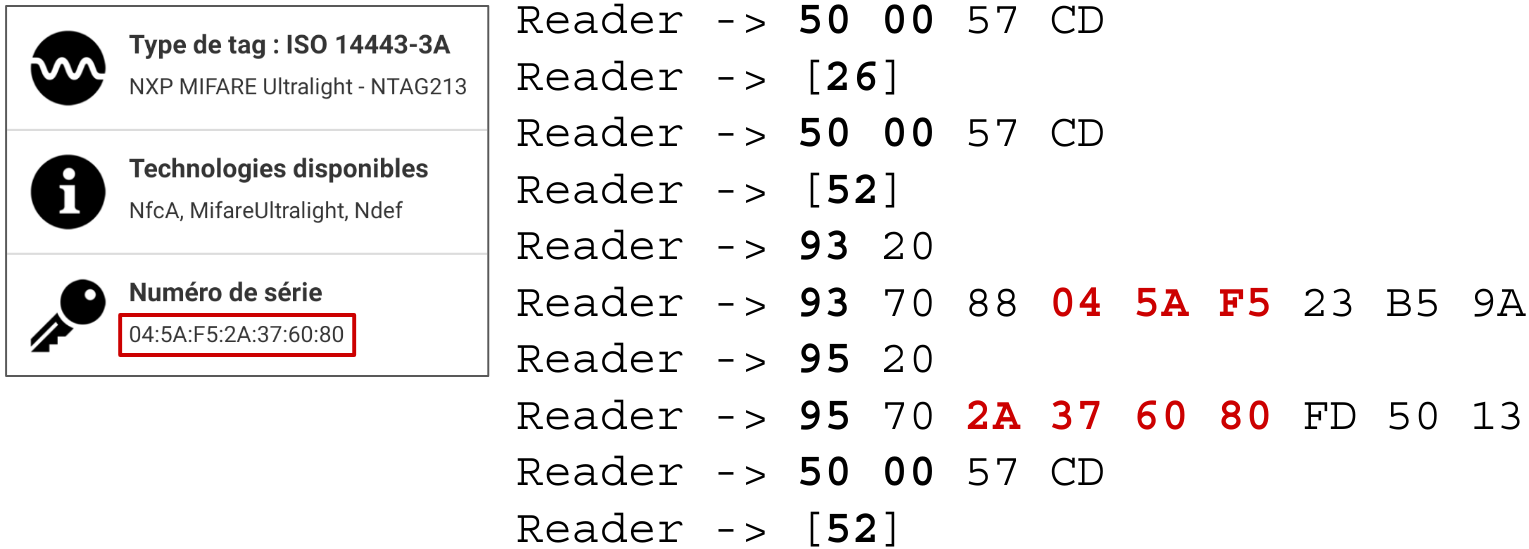
\includegraphics[scale=0.35]{figures/data_decoded-frames_app.png}
  \caption{Decoded frames from the reader, showing tag1's UID in red}
  \label{fig:decoded}
\end{figure}

At the time of this writing, we are investigating ways to decode the transmissions of both the reader and the tags. Using \texttt{sigrok}'s decoders\footnote{\url{https://sigrok.org/wiki/Protocol_decoders}} or Universal Radio Hacker\footnote{\url{https://github.com/jopohl/urh}}, we should be able to at least validate the signals, and maybe even decode them fully.
